\documentclass{article}
\usepackage[T1]{fontenc}
\usepackage[ngerman]{babel}
\usepackage[scaled]{helvet}
\usepackage{svg}
\renewcommand{\familydefault}{\sfdefault}

\usepackage{graphicx}


\title{Semesterleistung 1 AAI}
\date{31.3.2026}
\author{Salome Blum, HSLU}


\begin{document}

\maketitle

\paragraph{Vorbemerkung}
Es wurden mehrere Parameter-Konfigurationen für das Datenset CIFAR ausprobiert. Leider wurde mit den Eigenkonfigurationen eine Accuracy 
von maximal 0.79 erzielt. Das beste Resultat wurde mit der in der Aufgabenstellung vorgeschlagenen Parameterkonfiguration erzielt mit einer Accuracy von knapp 0.80.
Im Folgenden werden nur die Resultate der Standardkonfiguration gezeigt. 


\section{Angepasste 2D Ranking Funktion}

\begin{figure}[h]
\centering
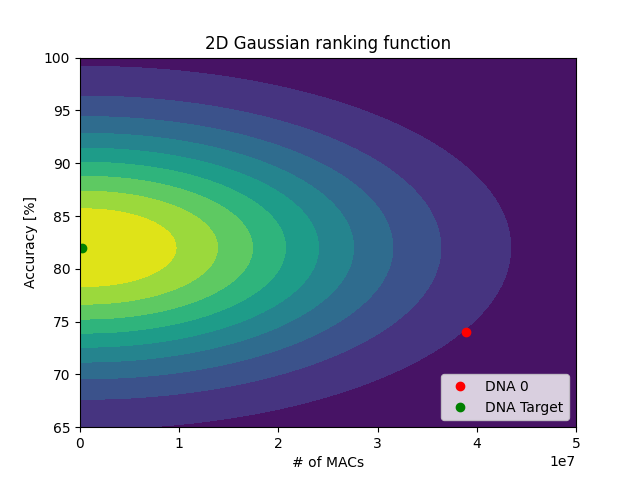
\includegraphics[width=0.8\textwidth]{img/2D_RankingPlot.png}
\caption{2D Ranking Plot}
\label{fig:rankingPlot}
\end{figure}

Der 2D-Ranking-Plot zeigt, dass der Gradient der zweidimensionalen Gauss’schen Rankingfunktion vom Referenz-DNA 0 aus in Richtung des Zielwerts verläuft. Es ist zu erwarten, dass die EAS die generierten Populationen in Richtung des Zielwerts optimiert.


\section{Evolution Plot}

\begin{figure}[h]
\centering
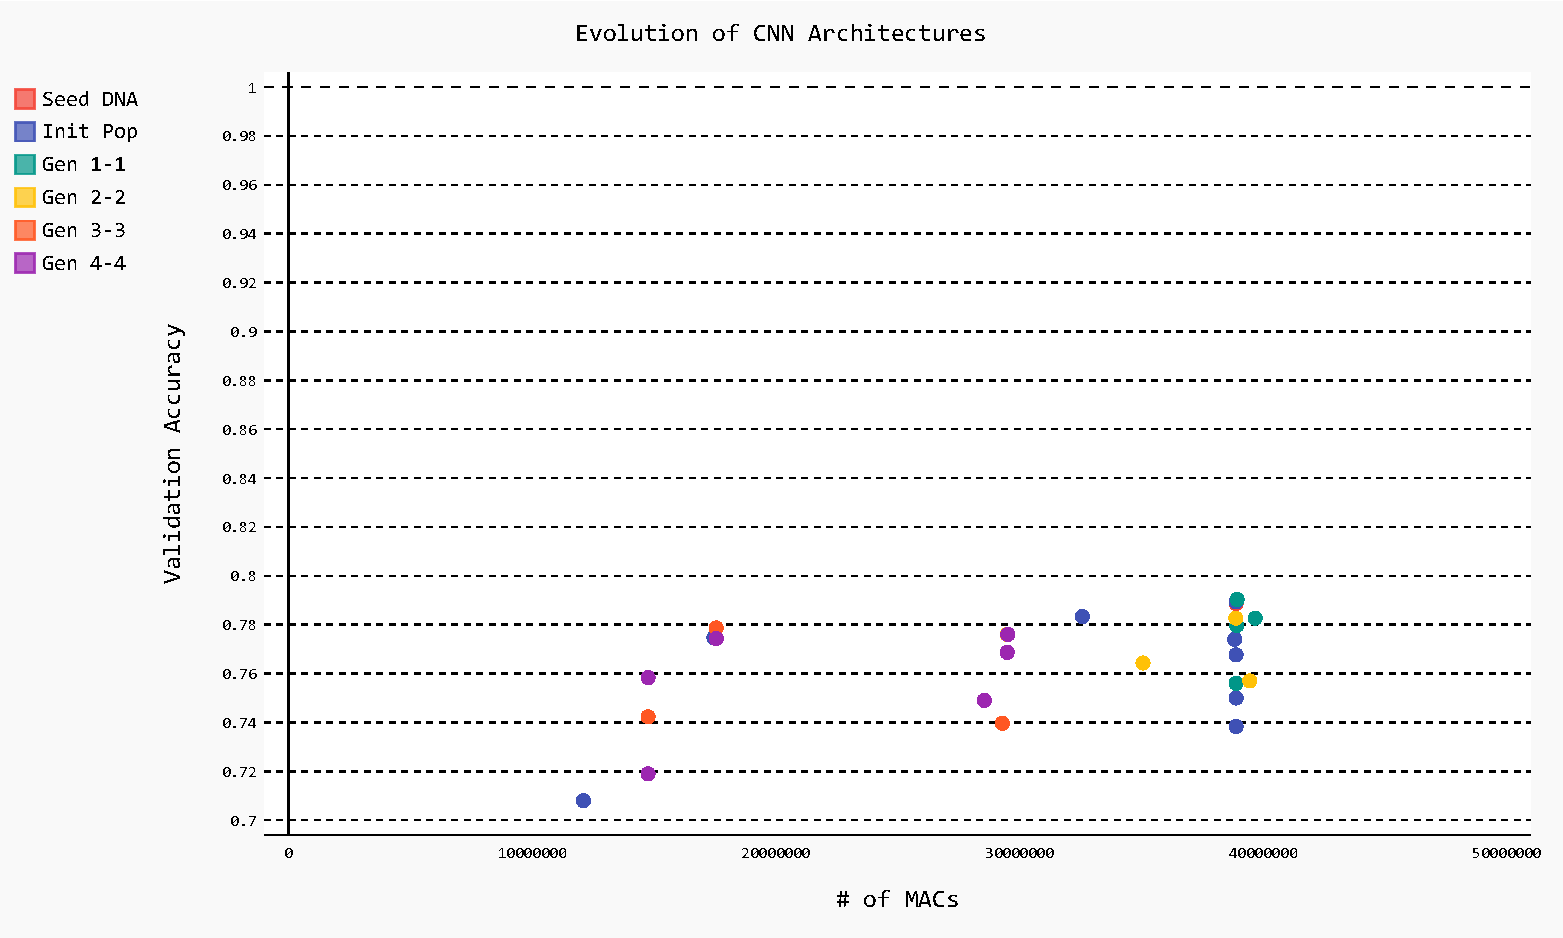
\includegraphics[width=0.8\textwidth]{img/CNN_evolution_2.pdf}
\caption{Evolution Plot}
\label{fig:evolutionPlot}
\end{figure}

Der CNN Evolutionsplot zeigt die vier Generationen der EAS. Dabei ist ersichtlich, dass die Anzahl MACs mit 
in den jüngeren Generationen deutlich abnimmt. Gleichzeitig nimmt auch die Accuracy ab, wobei in der Generation 3 ein Modell 
gefunden wurde, welches immerhin eine Accuracy von noch knapp 0.78 erreichte. Als Bestes Modell für das Retraining wurde DNA 11 aus der zweiten Generation 
gewählt, da es die beste Accuracy mit 0.79 hatte.

\section{Architektur der DNA 11}

\begin{figure}[h]
\centering
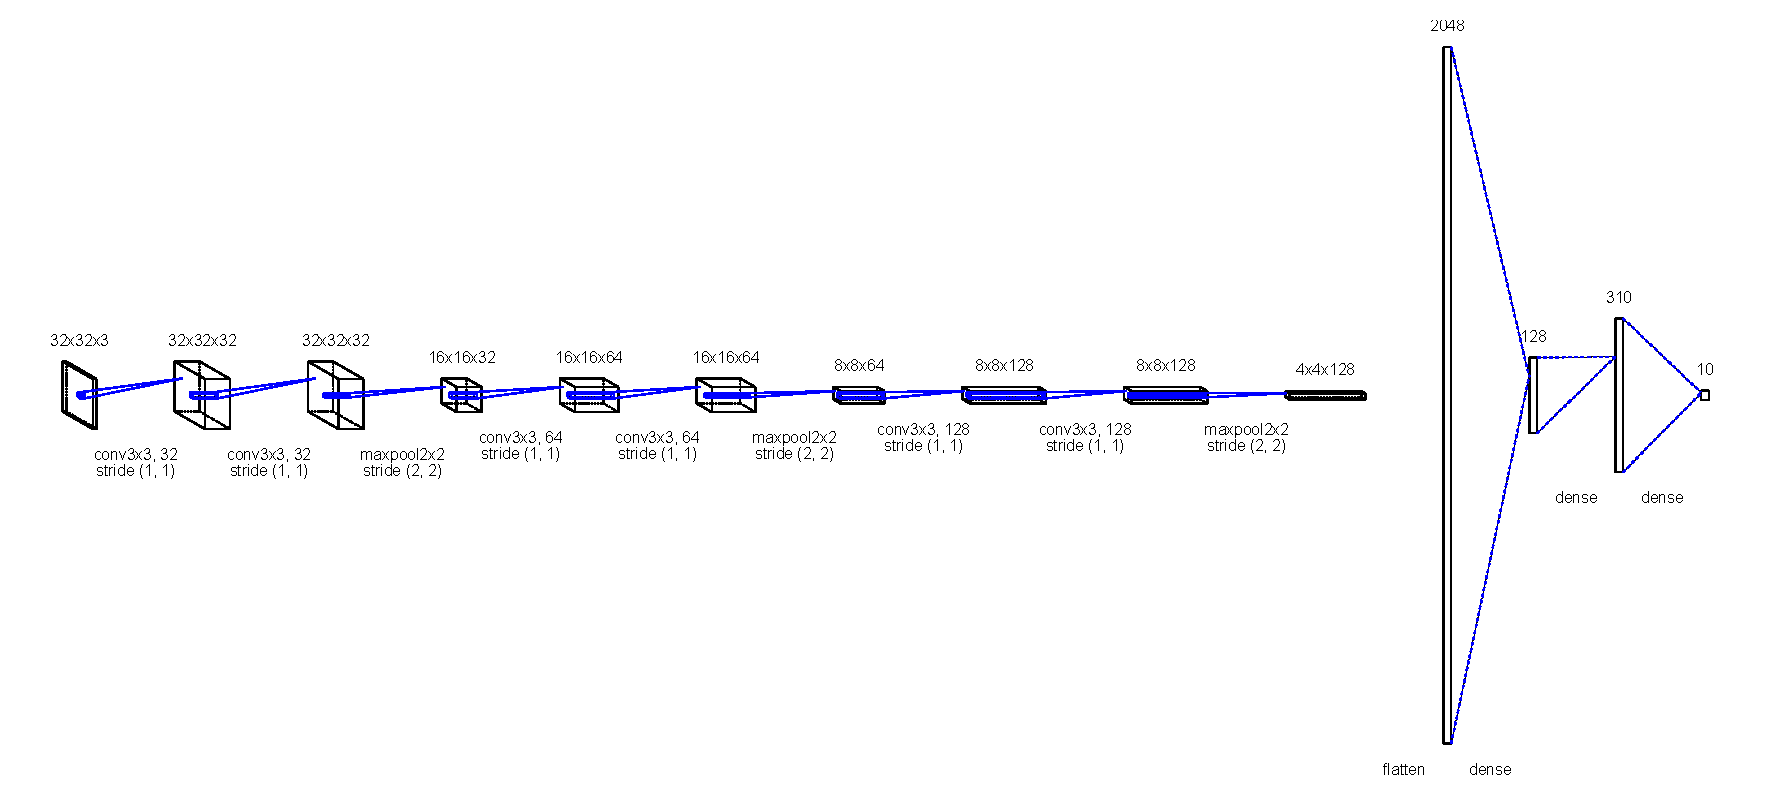
\includegraphics[width=0.8\textwidth]{img/Architecture_DNA_11.pdf}
\caption{Architektur DNA 11}
\label{fig:arch_dna11}
\end{figure}

\subsection{Berechnungen MAC Operationen und Weights}

\subsubsection{Conv Layer 1 - 32x32x3 --> 32x32x32}
N\_MACs = (32 × 32 × 32) × (3 × 3 × 3) = 884736 MACs
N\_Weights = (3 × 3 × 3) × 32 + 32 = 896 Weights

\subsubsection{Conv Layer 2 - 32x32x32 --> 32x32x32}
N\_MACs = (32 × 32 × 32) × (3 × 3 × 32) = 9'437'184 MACs
N\_Weights = (3 × 3 × 32) × 32 + 32 = 9248 Weights

\subsubsection{Maxpooling auf 16x16x32}

\subsubsection{Conv Layer 3 - 16x16x32 --> 16x16x64}
N\_MACs = (16 × 16 × 64) × (3 × 3 × 32) = 4'718'592 MACs
N\_Weights = (3 × 3 × 32) × 64 + 64 = 18'496 Weights

\subsubsection{Conv Layer 4 - 16x16x64 --> 16x16x64}
N\_MACs = (16 × 16 × 64) × (3 × 3 × 64) = 9'437'184 MACs
N\_Weights = (3 × 3 × 64) × 64 + 64 = 36'928 Weights

\subsubsection{Maxpooling auf 8x8x64}

\subsubsection{Conv Layer 5 - 8x8x64 --> 8x8x128}
N\_MACs = (8 × 8 × 128) × (3 × 3 × 64) = 4'718'592 MACs
N\_Weights = (3 × 3 × 64) × 128 + 128 = 73'856 Weights

\subsubsection{Conv Layer 6 - 8x8x128 --> 8x8x128}
N\_MACs = (8 × 8 × 128) × (3 × 3 × 128) = 9'437'184 MACs
N\_Weights = (3 × 3 × 128) × 128 + 128 = 145'584 Weights

\subsubsection{Maxpooling auf 4x4x128}

\subsubsection{FC Layer 1 - Flatten (4x4x128 = 2048) --> Dense(128)}
N\_MACs = 2048 × 128 = 262'144 MACs
N\_Weights = (2048 × 128) + 128 = 262'272 Weights

\subsubsection{FC Layer 2 - Dense (128) --> Dense(310)}
N\_MACs = 128 × 310 = 39'680 MACs
N\_Weights = (128 × 310) + 310 = 39'990 Weights

\subsubsection{FC Layer 3 - Dense (310) --> Dense(10)}
N\_MACs = 310 × 10 = 3'100 MACs
N\_Weights = (310 × 10) + 10 = 3'110 Weights

\subsubsection{Total}
Total MACs = 38'938'396 MACs\\
Total Weights = 592'380 Weights

\section{Vergleich DNA 0 mit DNA 11}
DNA 0 ist eine flache Startarchitektur ohne komplexe Layer und ohne Rechenaufwand. DNA 11 nutzt eine tiefere CNN-Struktur mit mehreren Conv-Layern, BatchNormalization
und Dropout. Dadurch kann liefert sie bessere Ergebnisse: 79\% (bzw. 81.7\% nach Retraining) im Vergleich zu den 74.1 \% der DNA 0. 
Allerdings benötigt sie dafür auch deutlich mehr Ressourcen. 

\begin{table}[h]
\centering
\caption{Vergleich der DNA-Konfigurationen}
\label{tab:dna_comparison}
\begin{tabular}{lcc}
\hline
\textbf{Merkmal} & \textbf{DNA 0} & \textbf{DNA 11} \\
\hline
Accuracy & 74.1\% & 79.0\% \\
MACs & 0 & 38.9 Mio \\
Weights & 0 & 592'380 \\
Generation & 0 & 1 \\
Mutation & 0 & 2 \\
Regularisierung & 0 & Dropout + BatchNorm \\
Convolutional Layer & 0 & 6 \\
FullyConnected Layer & 0 & 3 \\
\hline
\end{tabular}
\end{table}

\end{document}